\documentclass[a4paper,11pt,fleqn]{article}%fleqn pour aligner les equations à gauche
\usepackage{../../Styles/Cours}

\newcommand{\chnum}{Chapitre 13}
\newcommand{\chtitle}{Mouvement des satellites et planètes}
\newcommand{\dtype}{TP1}
  
\begin{document}
\maketitle

\section{Mouvement de la Terre}
\begin{enumerate}
    \item Expliquer à l'aide des données du document 1, pourquoi il est légitime, lors de l'étude des forces s'exerçant sur la Terre, de négliger les forces d'interaction gravitationnelle exercées par les planètes devant celle exercées par le Soleil.
    \item Préciser, pour l'étude du mouvement de la Terre : le référentiel, le système et les forces extérieures.
    \item A l'aide de la deuxième loi de Newton, déterminer l'expression vectorielle de l'accélération de la Terre en fonction de $m_S$ (masse du Soleil), $G$, $d_{ST}$ (distance Soleil-Terre). On utilisera le repère de Frenet.
    \item Donner deux adjectifs pour qualifier l'accélération de la Terre. En déduire la nature de son mouvement.
    \item En déduire la valeur de son accélération $a$ en fonction de la vitesse $v$ et de $d_{ST}$.
    \item Calculer la vitesse de la Terre. (donnée : $G=\SI{6,67E-11}{\meter\cubed\per\kilo\gram\per\second\squared}$)
    \item Calculer, en jours la période de révolution de la Terre autour du Soleil.
\end{enumerate}

\section{Les lois de Kepler}
\begin{minipage}{.7\linewidth}
On a représenté en noir sur le schéma ci-contre la portion d'aire balayée depuis le point $A$ durant une durée $\Delta t$.
\begin{enumerate}
    \item En utilisant la deuxième loi de Kepler (dans le cas général d'une trajectoire elliptique), représenter l'aide balayée pendant la durée $\Delta t$ à partir du point $B$.
\end{enumerate}
On appelle \emph{périgée} le point de l'orbite le plus proche de l'astre attracteur et \emph{apogée} le point de l'orbite le plus éloigné de l'astre attracteur.
\begin{enumerate}[resume]
    \item Expliquer quelle proposition parmi les trois ci-dessous est correcte :
    \begin{itemize}
        \item[\ding{114}] Les valeurs de la vitesse sont les mêmes au périgée et à l'apogée
        \item[\ding{114}] la vitesse est plus grande à l'apogée qu'au périgée
        \item[\ding{114}] la vitesse est plus grande au périgée qu'à l'apogée
    \end{itemize}
\end{enumerate}
\end{minipage}
\begin{minipage}{.3\linewidth}
    \centering
    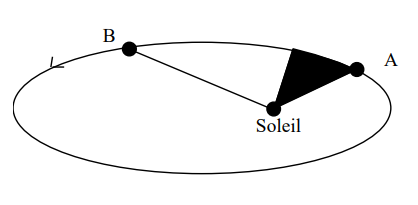
\includegraphics[width=\linewidth]{Ressources/TSPE_C10_AE1_Fig2.png}
\end{minipage}

\section{Satellites géostationnaires}
Un satellite \emph{géostationnaire} est un satellite terrestre restant en permanence à la verticale d'un même point à la surface de la Terre.

\begin{minipage}{.6\linewidth}
    \centering
    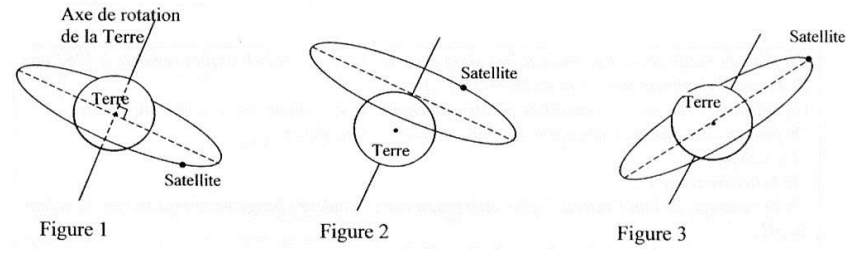
\includegraphics[width=\linewidth]{Ressources/TSPE_C10_AE1_Fig4.png}
\end{minipage}
\begin{minipage}{.4\linewidth}
\begin{enumerate}
    \item Expliquer quelle est la seule trajectoire possible pour un satellite géostationnaire.
    \item En déduire le lien entre sa période de révolution et période de rotation propre de la Terre.
    \item Déterminer l'altitude d'un tel satellite à l'aide de la troisième loi de Kepler.
\end{enumerate}
\end{minipage}

\begin{figure}[h!]
    \centering
    \caption*{\textbf{Document 1 : Le système solaire}}
    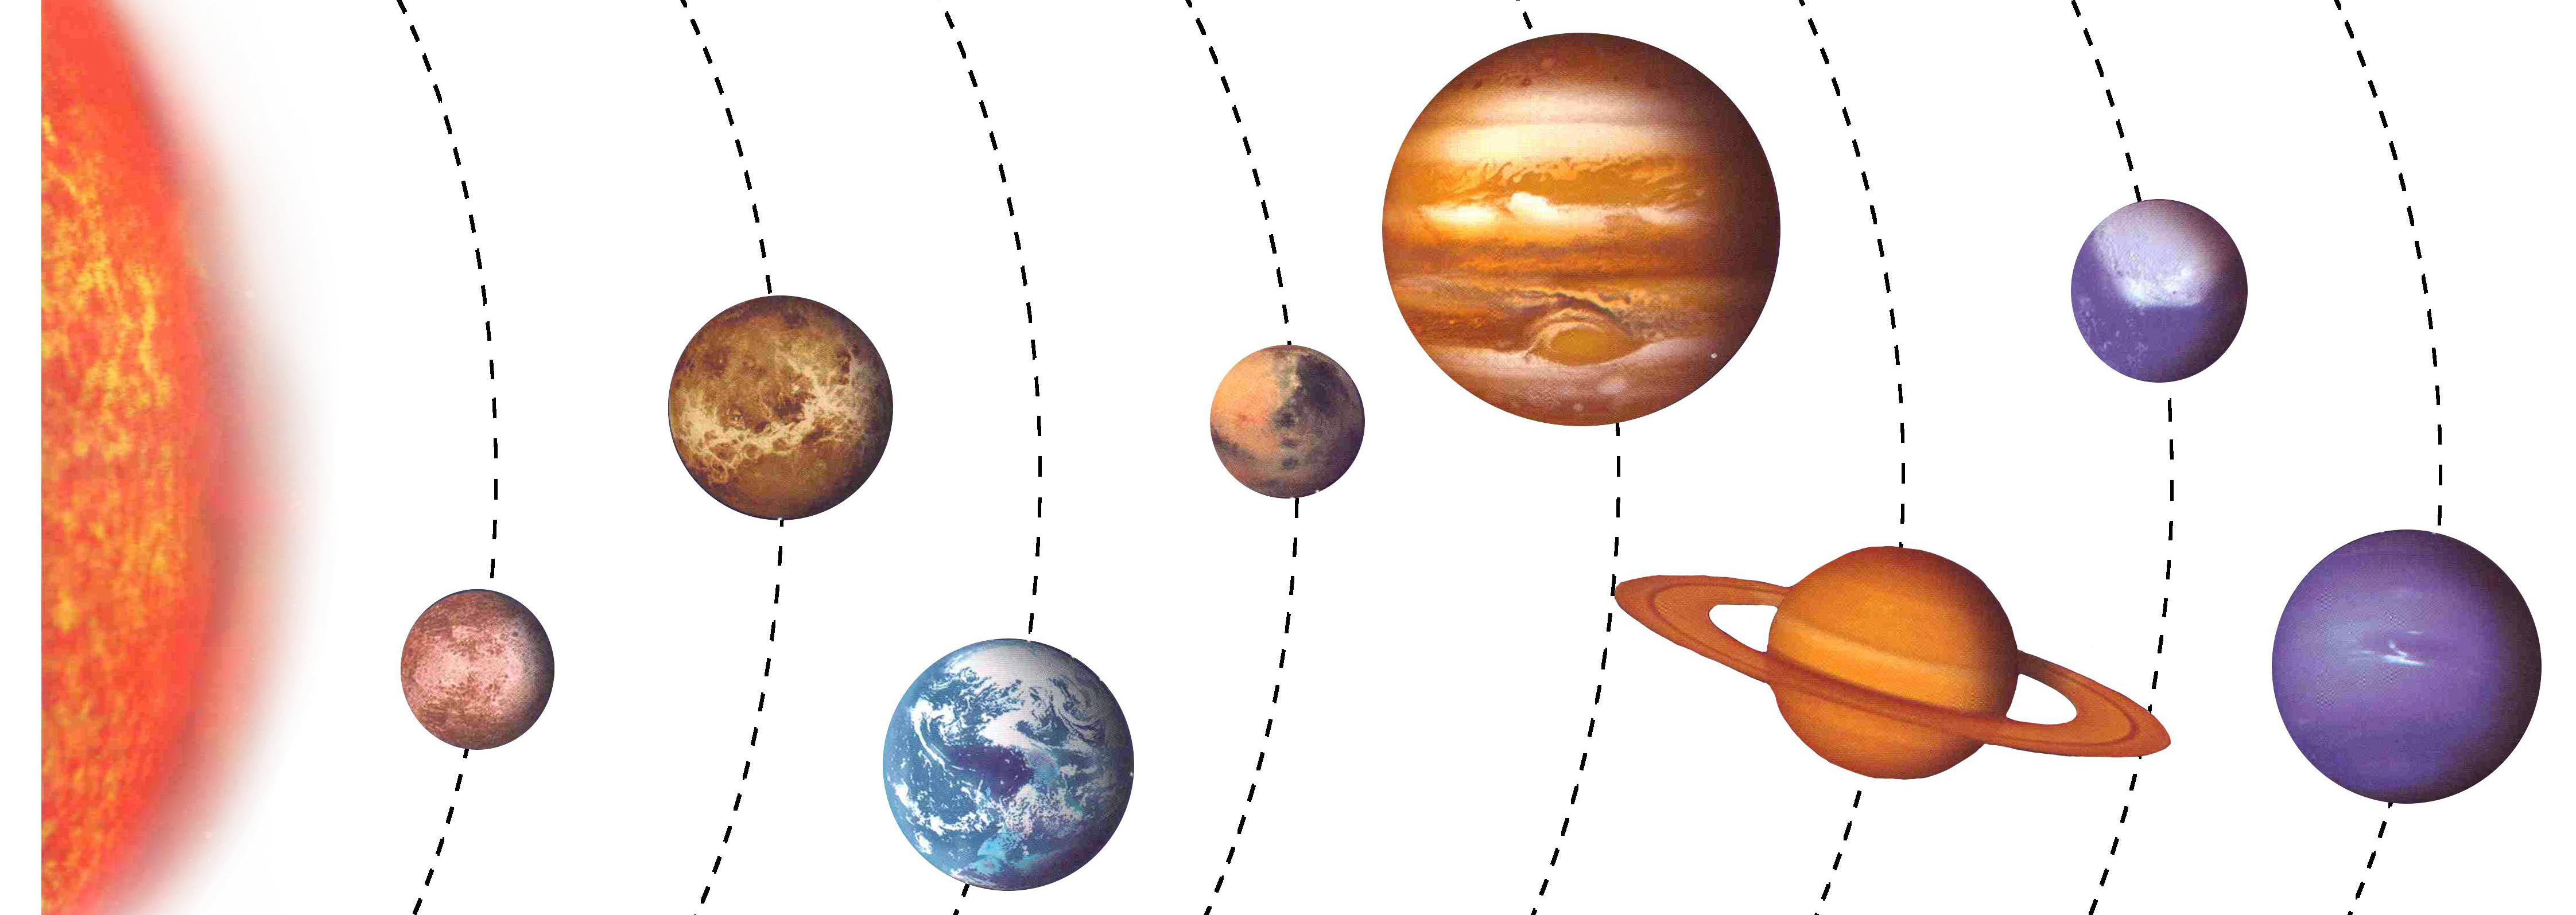
\includegraphics[width=1\linewidth]{Ressources/TSPE_C10_AE1_Fig1.png}
    \scriptsize
    \begin{tabular}{|c|c|c|c|c|c|c|c|c|} \hline
    Planète & Mercure & Vénus & Terre & Mars & Jupiter & Saturne & Uranus & Neptune\\ \hline
         Distance au Soleil (km)&\num{58E6}&\num{110E6}&\num{150E6}&\num{230E6}&\num{780E6}&\num{1400E6}&\num{2900E6}&\num{4500E6}\\ \hline
         Masse (kg)&\num{3,285E23}&\num{4,867E24}&\num{5,972E24}&\num{6,39E23}&\num{1,898E27}&\num{5,683E26}&\num{8,681E25}&\num{1,024E26}\\ \hline
    \end{tabular}
    \label{fig:doc1}
\end{figure}

\begin{figure}[h!]
    \caption*{\textbf{Document 2 : Les lois de Kepler}}
    \fbox{\begin{minipage}{.5\linewidth}
        \caption*{\textbf{Première loi de Kepler (ou loi des orbites, 1609)}}
        Les orbites des planètes sont des ellipses dont le Soleil occupe l'un des foyers.\\
        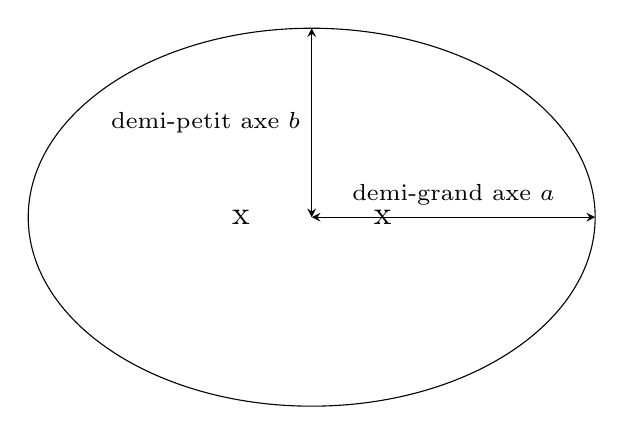
\begin{tikzpicture}[scale=1.2,transform shape]
            \draw (0,0) ellipse (3cm and 2cm);
            \draw[stealth-stealth] (0,0)to(3,0);
            \draw[stealth-stealth] (0,0)to(0,2);
            \draw (1.5,0) node[above]{\scriptsize demi-grand axe $a$};
            \draw (0,1) node[left]{\scriptsize demi-petit axe $b$};
            \node (F1) at (-.75,0){x};
            \node (F2) at (.75,0){x};
        \end{tikzpicture}
    \end{minipage}}
    \fbox{\begin{minipage}{.49\linewidth}
        \caption*{\textbf{Deuxième loi de Kepler (ou loi des aires, 1609)}}
        Le segment reliant la planète en orbite au Soleil balaie des aires égales pendant des durées égales.\\
        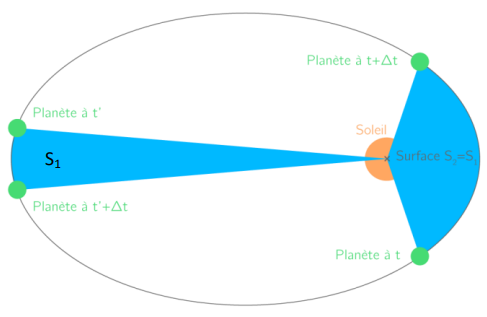
\includegraphics[width=.8\linewidth]{Ressources/TSPE_C10_AE1_Fig3.png}
    \end{minipage}}
    
    \fbox{\begin{minipage}{\linewidth}
        \caption*{\textbf{Troisième loi de Kepler (ou loi des périodes, 1618)}}
        Toutes les planètes en orbite autour d'une même étoile ont un rapport constant $\dfrac{T^2}{a^3}$ \\
        où $a$ est le demi-grand axe de l'orbite\\
        $T$ est la période de révolution de la planète
    \end{minipage}}
    
    \label{fig:doc2}
\end{figure}
\end{document}